\chapter{Анализ и идентификация физической реализации системы Колпитца}
\label{atu:ch:colpreal}

\section{Отличия реального генератора Колпитца}


Как уже было отмечено,
рассмотренная в разделе \ref{atu:sect:colp} модель
генератора Колпитца, несмотря на её широкое использование
при исследованиях, связанных с хаотической динамикой,
имеет существенные отличия от реального генератора.
Подавляющие большинство элементов достаточно хорошо описываются линейным
приближением. Однако, есть два элемента,
применение линейной модели для которых или же вообще невозможно (транзистор),
или же допустимо при определённых условиях (индуктивность).





\section{Физическая реализация генератора Колпитца и исследование её динамики}

На рис.~\ref{atu:f:colp_schem_real} представлена электрическая схема
реализации генератора Колпитца, используемая в данной работе.
Отличия от схемы, используемой в главе \ref{atu:ch:testsys}
и представленной на рис.~\ref{atu:f:colp_schem}
не принципиальны с точки зрения модели,
и предназначены как для упрощения подключения
измерительных устройств, так и для
обеспечения стабильности определённых потенциалов схемы.

\begin{figure}[htb!]
\centerline{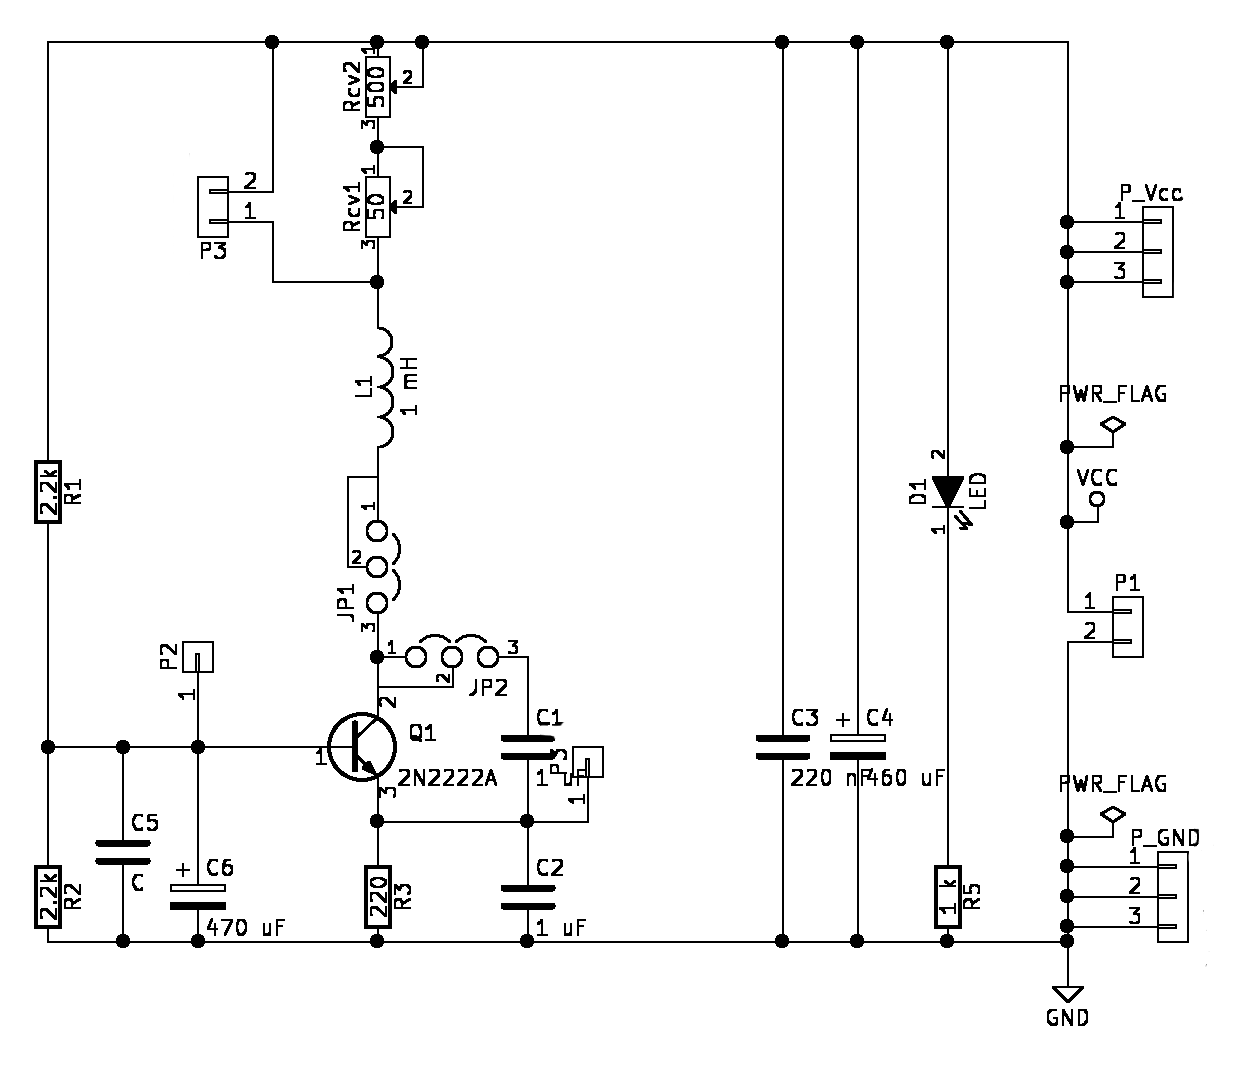
\includegraphics[width=0.7\textwidth]{p/colp_schem_real.png} }
\caption{Электрическая схема реального генератора Колпитца, используемого в данной работе}
\label{atu:f:colp_schem_real}
\end{figure}

Картинка платы.

Описание дополнительных элементов.

Недостатки использования осцилла -- что вместо

Примеры динамики с сравнением.

\section{Численная модель генератора Колпитца}

Методы расчёта~\cite{zaeplnii_radio_calc}.

\section{Анализ и выбор критериев}

Проверяем старые.

Исследуем всякие.

\begin{figure}[htb!]
\centerline{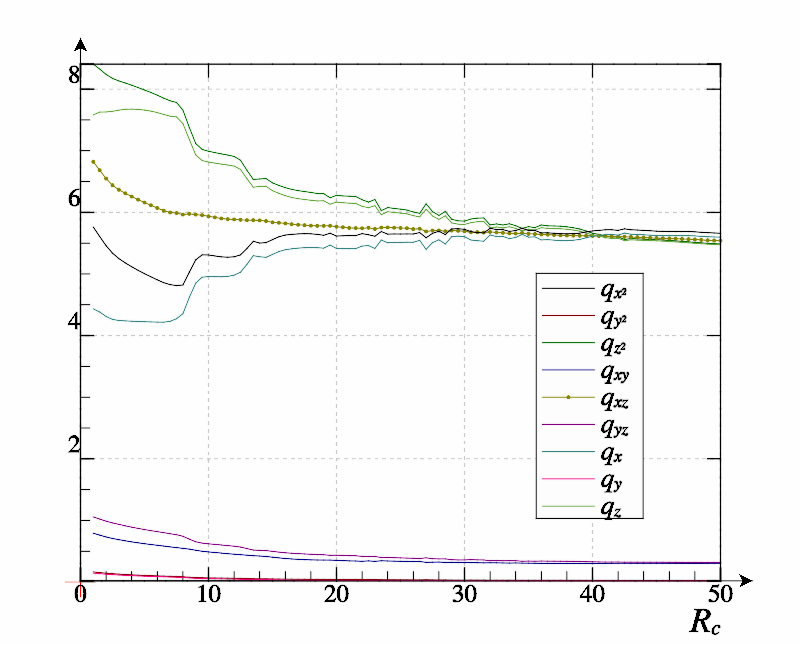
\includegraphics[width=0.7\textwidth]{p/colp_bjt_q-p_Rc_q.png} }
\caption{Зависимости значений критерия идентификации для системы Колпитца}
\label{atu:colp_bjt_q-p_Rc_q}
\end{figure}

Предлагаем новые.

\section{Синтез и анализ и системы идентификации}

Описание с картинкой.

Приметы процессов идентификации.

\begin{figure}[htb!]
  \centerline{
    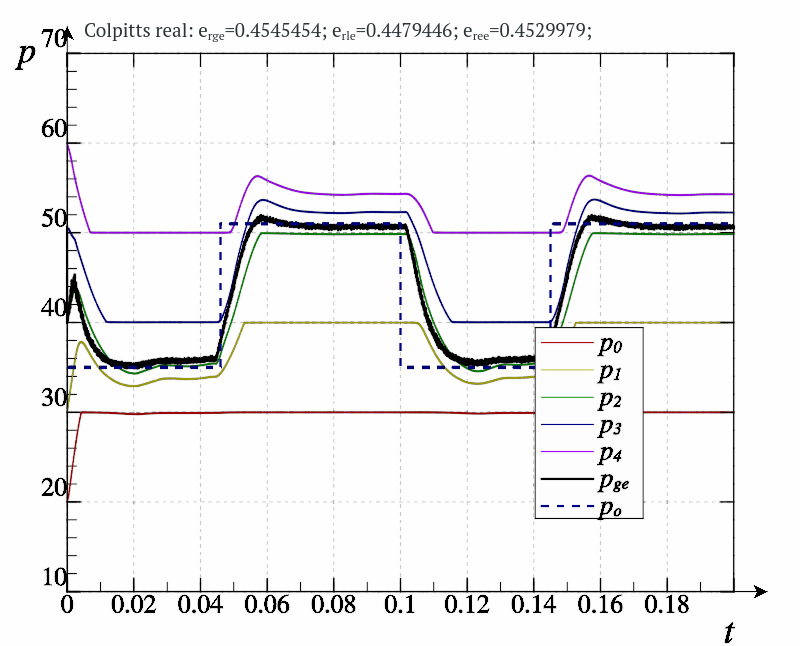
\includegraphics[width=0.48\textwidth]{p/colp_real_id_qi_fv5-p_p_01.png}
    \hfill
    \includegraphics[width=0.48\textwidth]{p/colp_real_id_qi_fv5-p_pp_01.png}
  }
  \caption{Процесс идентификации параметра $R_c$ реального генератора Колпитца '' при условиях }
  \label{atu:f:colp_r_id_1}
\end{figure}

Зависимости

\section{Выводы по разделу \thechapter}

Выводы.

